\documentclass[conference]{IEEEtran}
\usepackage[utf8]{inputenc}
\usepackage[T1]{fontenc}
\usepackage{amsmath,amssymb}
\usepackage{graphicx}
\usepackage{booktabs}
\usepackage{multirow}
\usepackage{xcolor}
\usepackage{tikz}
\usetikzlibrary{arrows.meta,positioning,fit,backgrounds}
\usepackage[hidelinks]{hyperref}
\usepackage{cite}
\graphicspath{{figs/}}
\definecolor{cblue}{HTML}{2A78D6}
\definecolor{corange}{HTML}{EB6834}
\definecolor{cgreen}{HTML}{1BAF7A}
\definecolor{cgray}{HTML}{52514E}
\newcommand{\RQ}[1]{\textbf{RQ#1}}

\begin{document}
\title{From 0.13 to 0.20: Trace-Guided Improvement of a Small Open-Weight Coding Agent under a Fixed Compute Budget}

\author{\IEEEauthorblockN{Muhammad Husnain Rasool}
\IEEEauthorblockA{CS594/794 Deep Learning --- Final Project Report\\ Nazarbayev University}
\and
\IEEEauthorblockN{Galymzhan Zaharas}
\IEEEauthorblockA{CS594/794 Deep Learning --- Final Project Report\\ Nazarbayev University}}

\maketitle

\begin{abstract}
Large language model (LLM) agents that repair real software issues are usually studied with frontier models, unlimited compute and test-based patch selection. We study the opposite regime: an open-weight model (Gemma~4 31B and E4B, 4-bit quantized) running inside a fixed compute budget, as in the Kaggle \emph{Gemma~4 Developer Agent} competition, where about 120 hidden GitHub issues must be solved on four L4 GPUs within 12 hours. Starting from the public \emph{Budget-Fit} agent (47.9 of 118 local tasks; 0.13 on the hidden leaderboard), we build a reproducible grader for the competition harness, run more than 15,000 agent episodes, and improve the agent step by step under a pre-registered screen--confirm protocol. Our final agent, \emph{Patchsmith-check}, solves \textbf{51.9} tasks ($+4.0$ [$+0.9$, $+7.2$], paired bootstrap), cuts runs wasted on budget limits by 71\% (9.2$\rightarrow$2.7 per seed), and raises the hidden leaderboard score from \textbf{0.13 to 0.20} (+54\% relative). Four research questions explain where the gain comes from and where it does not: (i) one evaluation carries about $\pm$5 tasks of seed noise, so 3--12 seeds and paired tests are needed; (ii) a larger per-run budget matches or beats sampling plus test-free selection at every measured cost, and selector gains halve on held-out seeds; (iii) three LoRA fine-tuning recipes (self-training, distillation from a stronger Qwen model, down-distillation to E4B) all \emph{reduce} accuracy, each for a diagnosable reason; and (iv) a within-task contrast of solved and failed traces yields a four-sentence prompt change that raises the targeted behaviours (pytest as final check 9\%$\rightarrow$27\%) and gives the final step of the improvement.
\end{abstract}

\begin{IEEEkeywords}
LLM agents, software engineering, test-time compute, LoRA, distillation, evaluation noise, Gemma
\end{IEEEkeywords}

%=========================================================
\section{Introduction}
LLM-based software engineering (SWE) agents read an issue, explore a repository through tools, edit code and submit a patch that is judged by hidden unit tests~\cite{jimenez2024swebench}. Progress on benchmarks such as SWE-bench has come largely from frontier models, from agent--computer interfaces~\cite{yang2024sweagent,wang2024openhands}, from pipelines that generate many candidate patches and pick one with tests~\cite{xia2024agentless,ehrlich2025codemonkeys}, and from training on large sets of verified trajectories~\cite{pan2025swegym,yang2025swesmith}.

Many practical settings look different: the model must be \emph{open and local}, compute is \emph{fixed}, and no test oracle is available at selection time. The Kaggle \emph{Gemma~4 Developer Agent} competition is a clean instance of this regime. Entrants submit only an agent configuration (prompt, tools, sampling and limits) for the organisers' harness; the organisers run it with Gemma~4~\cite{gemma2024,gemma3} on about 120 hidden GitHub issues on 4$\times$L4 GPUs within 12 hours, and rank by the fraction of issues whose hidden tests pass. A separate prize exists for the small Gemma~4 E4B/E2B models.

\paragraph*{Motivation} Within such a budget, a practitioner has three families of levers: (1) \emph{test-time compute} --- spend the budget on longer runs or on several runs plus selection~\cite{brown2024monkeys,snell2024scaling}; (2) \emph{weights} --- fine-tune the model, e.g.\ with LoRA~\cite{hu2022lora} on successful trajectories~\cite{zelikman2022star,yuan2023rft,chen2023fireact}; and (3) \emph{agent design} --- prompts, tools and control flow~\cite{yao2023react,yang2024sweagent}. Which of these actually moves a small agent, and how can one tell when single evaluations are noisy~\cite{kapoor2024agents,miller2024errorbars}?

\paragraph*{Research questions}
\begin{itemize}
\item \RQ{1} (\emph{measurement}): How noisy is one agent evaluation, and how many seeds are needed to detect a given improvement?
\item \RQ{2} (\emph{test-time compute}): At a fixed, \emph{measured} compute cost, is it better to give one run a larger budget or to sample several short runs and select a patch without tests?
\item \RQ{3} (\emph{fine-tuning}): Does LoRA fine-tuning on successful trajectories --- the model's own, a stronger teacher's, or the large model's for the small one --- improve the agent under competition constraints?
\item \RQ{4} (\emph{trace-guided design}): Can a statistical analysis of solved versus failed traces yield a targeted intervention that improves the agent, and does the gain transfer to the hidden leaderboard?
\end{itemize}

\paragraph*{Contributions}
(0) An improved agent: from the public Budget-Fit baseline to Patchsmith-check, $+4.0$ local tasks [$+0.9$, $+7.2$], 71\% fewer wasted runs, and 0.13$\rightarrow$0.20 on the hidden leaderboard (§\ref{sec:overall}); (1) a rootless, reproducible grader for the competition harness that fixes three silent scoring faults (§\ref{sec:data}); (2) a task-level noise model giving the minimum detectable difference per number of seeds (§\ref{sec:rq1}); (3) a matched-cost frontier over four budget regimes with a pre-registered selector holdout (§\ref{sec:rq2}); (4) three controlled LoRA experiments with a failure diagnosis for each (§\ref{sec:rq3}); (5) a trace-guided prompt intervention validated by a pre-registered screen/confirm protocol and by the hidden leaderboard (§\ref{sec:rq4}).

%=========================================================
\section{Related Work}
\paragraph*{SWE agents} SWE-bench~\cite{jimenez2024swebench} established repository-level issue resolution judged by hidden tests. SWE-agent~\cite{yang2024sweagent} showed that the agent--computer interface (file viewer, edit command, linting) matters as much as the model; OpenHands~\cite{wang2024openhands} generalised this into an open platform. Agentless~\cite{xia2024agentless} replaced the free-form loop by a fixed localise--repair--validate pipeline. All build on the ReAct pattern of interleaved reasoning and tool calls~\cite{yao2023react} and on chain-of-thought reasoning~\cite{wei2022cot}; Gemma~4 additionally exposes an explicit ``thinking'' channel with a token budget, in the spirit of reasoning-trained models such as DeepSeek-R1~\cite{deepseek2025r1}.

\paragraph*{Test-time compute} Repeated sampling raises the probability that \emph{some} sample is correct roughly log-linearly in the number of samples~\cite{brown2024monkeys}, and self-consistency selects by majority vote~\cite{wang2023selfconsistency}. Snell et al.~\cite{snell2024scaling} show that the compute-optimal allocation depends on difficulty. For SWE tasks, CodeMonkeys~\cite{ehrlich2025codemonkeys} and SWE-Gym~\cite{pan2025swegym} select among samples with generated tests or trained verifiers. We remove both, which is the realistic case for a small local agent.

\paragraph*{Fine-tuning agents} LoRA~\cite{hu2022lora} and QLoRA~\cite{dettmers2023qlora} make adaptation of large models affordable; LoRA learns less than full fine-tuning but forgets less~\cite{biderman2024lessforgets}. Training on a model's own filtered successes goes back to STaR~\cite{zelikman2022star} and rejection-sampling fine-tuning~\cite{yuan2023rft}; FireAct~\cite{chen2023fireact} and AgentTuning~\cite{zeng2023agenttuning} distil stronger models' agent trajectories. SWE-Gym~\cite{pan2025swegym} and SWE-smith~\cite{yang2025swesmith} train SWE agents on hundreds to tens of thousands of verified trajectories. Imitation can copy style rather than capability~\cite{gudibande2023false}, and likelihood training can produce repetition loops~\cite{holtzman2020degeneration}; we observe both.

\paragraph*{Evaluation} Kapoor et al.~\cite{kapoor2024agents} argue for cost-aware agent comparison; Miller~\cite{miller2024errorbars} for error bars on LLM evaluations. We apply both to a live competition and quantify how far a public leaderboard can be trusted.

%=========================================================
\section{Data and Problem Setting}\label{sec:data}
\paragraph*{Task} Each task is a real GitHub issue with a repository snapshot. The agent operates in a sandbox with tools \texttt{run\_command}, \texttt{read\_file}, \texttt{edit\_file}, \texttt{write\_file}, \texttt{get\_status} and \texttt{submit\_patch}; its final diff is graded by the repository's hidden tests (\texttt{FAIL\_TO\_PASS} and \texttt{PASS\_TO\_PASS}). Formally, the agent is a policy $\pi_\theta$ over a partially observed environment: at step $i$ the model generates a thought $z_i$ and a tool call $a_i \sim \pi_\theta(\cdot \mid x, z_{<i}, a_{<i}, o_{<i})$ and receives observation $o_i$; the episode ends at submission or when a limit is hit. The entrant controls the prompt $x$, the tool set, the sampling parameters and three limits per task (wall time, tool calls, model turns); $\theta$ can only be changed through a LoRA adapter.

\paragraph*{Data} The competition releases 129 public tasks from four Python repositories (fastapi, rich, requests, httpx), each with the issue text, optional hints, a gold patch and the hidden tests; the leaderboard uses about 120 hidden tasks of the same kind (public split $\approx$58 tasks). We applied the gold patch and an empty patch to every task: gold resolves 120/129 and empty 2/129, leaving \textbf{118 sound tasks} (fastapi 60, rich 45, requests 12, httpx 1). For fine-tuning we additionally hold out 24 tasks (§\ref{sec:rq3}).

\paragraph*{Grader} The harness expects Docker; our cluster allows only rootless Apptainer. We wrote a drop-in container manager and found three faults in the public setup that change scores silently: (1) bundled wheels of the target projects shadowed the repository under test (38 tasks ``passed'' with an empty patch); (2) installing the newest of many dependency versions (56 of starlette) broke old snapshots --- we choose, per task, the newest version allowed by the repository's constraints \emph{and} released before the issue date; (3) a fixed-name cache in \texttt{/tmp} made concurrent jobs reuse wrong environments. After the fixes the grader reproduces official labels on gold and empty patches.

\paragraph*{Model and serving} Gemma~4 31B and E4B in the competition's quantization-aware-trained 4-bit weight / 16-bit activation (QAT w4a16) checkpoints, served by vLLM~\cite{kwon2023vllm}. Kaggle uses a \emph{patched} vLLM 0.19.1 wheel; we installed that exact wheel on our cluster (2$\times$H100 per server, tensor parallel 2, 10 concurrent tasks). Sampling uses temperature 0.2, top-$p$ 0.95, a 4,096-token thinking budget and at most 8,192 output tokens per step. A 26-task Kaggle notebook run showed L4 agent time to be 1.17$\times$ H100 time, which we use to project Kaggle runtime: $T_\text{Kaggle}\approx 1.17\cdot 120\cdot \bar t_\text{H100}$.

\begin{figure*}[t]
\centering
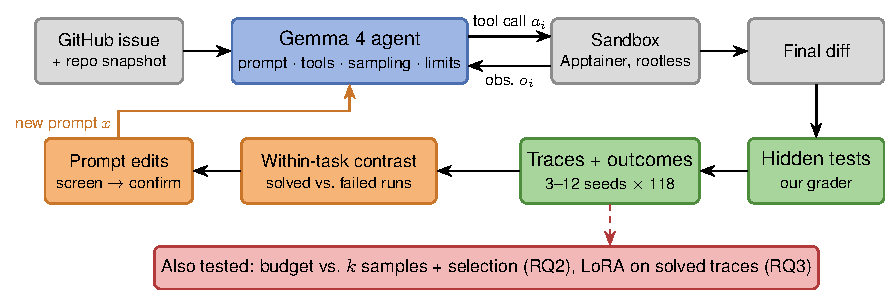
\includegraphics[width=0.86\textwidth]{v2/fig_pipeline.pdf}
\caption{Experimental pipeline and improvement loop. Every configuration runs with several seeds on all 118 tasks; our grader scores the final diff; solved and failed traces of the same task are contrasted, and the resulting prompt edits pass a screen and a fresh-seed confirmation before adoption (orange). Red: other levers we tested (RQ2, RQ3).}
\label{fig:pipeline}
\end{figure*}

%=========================================================
\section{Methodology}
\subsection{Baseline and improvement path}\label{sec:baseline}
\textbf{Baseline.} Our starting point is \emph{Budget-Fit}, the public 31B configuration the competition community regarded as the most stable (8\,min / 28 tool calls / 80 turns per task, temperature 0.2). Every later step is compared with it: 47.9 tasks over 10 seeds locally and 0.13 on the hidden public leaderboard. \textbf{Path.} Each candidate change keeps the competition limits, is run on all 118 tasks with 3--12 seeds, and is compared with its predecessor by the paired test below. In order: (1) a \emph{budget guard} we added to the prompt (stop exploring and edit by a fixed call); (2) \emph{pub\_v6}, a public prompt claimed to score 0.24; (3) \emph{Patchsmith}, the strongest public workflow we found (reproduce--edit--check); (4) \emph{Patchsmith-check}, our trace-guided revision of Patchsmith (§\ref{sec:rq4}). Steps (2) and (3) are adopted public configurations and steps (1) and (4) are our own; Table~\ref{tab:path} keeps this distinction.

\subsection{Statistical protocol (all RQs)}
Let $s^{A}_{t,k}\in\{0,1\}$ be whether configuration $A$ solves task $t$ with seed $k$. We report the mean number solved per seed, $\bar S_A = \sum_t \bar s^A_t$ with $\bar s^A_t$ the per-task mean over seeds. Differences are $\Delta = \sum_t(\bar s^A_t-\bar s^B_t)$ with a 95\% interval from a paired bootstrap over tasks (5,000--10,000 resamples). For the noise model we treat each task as a Bernoulli trial with its own resolve probability $p_t$, so that one run's score has variance
\begin{equation}
\sigma^2 = \sum_{t} p_t (1-p_t), \qquad \text{MDE}(n) = (z_{0.975}+z_{0.8})\sqrt{2\sigma^2/n},
\end{equation}
the minimum detectable difference with $n$ seeds per arm at 95\% confidence and 80\% power. To avoid the winner's curse, candidate changes follow a \emph{screen--confirm} protocol fixed in advance: a 3-seed screen with a gate, then fresh seeds for confirmation, and adoption only if the pooled difference clears a pre-set bar.

\subsection{RQ2: budget versus sampling}
Four budget regimes: short (8\,min / 28 calls / 80 turns, the starter default), medium (16 / 56 / 160), long (40 / 140 / 400) and long with a budget-aware prompt; 2,950 runs in total. \emph{Cost} is what runs actually spent (agent minutes; generated tokens give the same ratios), not the nominal limit. A $k$-sample strategy costs the sum of its $k$ runs and picks one patch with a test-free selector using only the patch and trace: a validity filter (drop runs that changed no source file or hit a limit), trace signals (exit code of the last command after the final edit, patch size), patch consensus, and Gemma~4 as a pointwise (0--10) or listwise judge. The best rule found on seeds 0--4 was frozen in a written pre-registration and re-tested on seeds 5--9.

\subsection{RQ3: LoRA on successful trajectories}
\textbf{Data.} From 4,130 earlier 31B runs, solved runs exist for 70 tasks; 24 of these (stratified by repository) are held out. \emph{Self:} up to four solved runs per task (fewest calls, no stray files), 169 episodes from 46 tasks. \emph{Teacher:} Qwen3.6-35B-A3B run as the agent in the same harness (it solves 52/118 with 60 calls vs.\ 49.0 for 31B), solved runs with $\le$28 calls, parallel calls split into single calls, 126 episodes from 39 tasks. \emph{Down-distillation:} the self data used to train E4B.
\textbf{Rendering and loss.} Episodes are rendered with Gemma's chat template with thinking enabled, so earlier thoughts appear exactly as at inference. The loss is the token-level negative log-likelihood restricted to the model's own spans,
\begin{equation}
\mathcal{L}(\phi) = -\sum_{j \in \mathcal{M}} \log p_{\theta+\Delta\phi}(y_j \mid y_{<j}),
\end{equation}
where $\mathcal{M}$ covers each model turn up to and including its stop token (\texttt{<|tool\_response>} or \texttt{<turn|>}). Because full episodes (up to 27k tokens) did not fit in memory and efficient attention kernels did not support Gemma~4's 512-dimensional global heads, episodes are split into 8,192-token windows holding the system prompt, the task, up to three earlier turns as unsupervised context and a block of supervised turns; each turn is trained once.
\textbf{Recipe.} LoRA~\cite{hu2022lora} with $W = W_0 + \tfrac{\alpha}{r}BA$, rank $r=16$, $\alpha=32$, dropout 0.05, on all attention and MLP projections (122M trainable parameters, 0.38\% of 31B; 35M for E4B). QAT weights are decompressed to bfloat16. AdamW, learning rate $10^{-4}$, cosine schedule, 5\% warm-up, clipping 1.0, 16 windows per step, 2 epochs (31B self: 106 steps, 7.8\,h on 4$\times$H100). Adapters are served with Kaggle's vLLM wheel, which --- unlike the public release of the same version --- accepts LoRA on Gemma~4.

\subsection{RQ4: trace-guided intervention}
\textbf{Baseline.} \emph{Patchsmith}, the strongest public 31B configuration we tested (50.2 solved over 12 seeds vs.\ 47.5 for the previous public best; Kaggle 0.17).
\textbf{Analysis.} On 708 Patchsmith runs we (a) localised each failed patch against the gold patch by mapping diff hunks to functions with Python's AST, (b) computed per-run behavioural features from the traces (first edit call, reproduction before editing, behaviour check after the last edit, pytest use, scratch files, edit loops), (c) estimated each feature's effect \emph{within task}: on the 29 ``mixed'' tasks that are solved by some seeds and not others, we compare solved and failed runs of the \emph{same} task, which removes task difficulty as a confounder, and report the paired effect size $d_z$, and (d) manually audited 30 failed runs sampled stratified by repository and seed.
\textbf{Intervention.} Only features that separate outcomes within task and are under-used become prompt changes. The resulting \emph{Patchsmith-check} changes four sentences of the system prompt and nothing else (limits, tools and sampling identical): it states that pytest works in the sandbox (with a fallback if it does not), adds a four-step final checklist (compile all changed files after the last edit; rerun one's reproduction unchanged; run the most relevant existing test file with \texttt{pytest -x -q}; fix and recheck), adds an edit-retry rule, and directs scratch files to \texttt{/tmp}.
\textbf{Gates (fixed in advance).} Screen (3 seeds): $\Delta\ge+1$, time per task $\le$235\,s, and a clear rise in post-edit checking. Confirm (6 fresh seeds of both): pooled $\Delta\ge+1.5$, held-out tasks no worse, projected Kaggle time $\le$11.5\,h, and a robustness seed with pytest disabled within one task of the baseline.

%=========================================================
\section{Results and Analysis}
\subsection{Overall: from the baseline to our final agent}\label{sec:overall}
Table~\ref{tab:path} and Fig.~\ref{fig:overview} summarise the improvement path. The final agent solves 51.9 tasks per seed against 47.9 for the Budget-Fit baseline, $+4.0$ [$+0.9$, $+7.2$], an interval that excludes zero. The main mechanism is the one the rest of this report identifies: fewer wasted runs. Runs stopped by a time, call or turn limit fall from 9.2 to 2.7 per seed (Fig.~\ref{fig:overview}b) while time per task stays the same (228 vs.\ 222\,s), so the projected Kaggle time remains 8.7\,h. On the hidden leaderboard the score rises monotonically from 0.13 to 0.20; each single step is within leaderboard noise (SD 0.048), but the full path is 1.5 SD. About 60\% of the local gain comes from adopting the Patchsmith workflow ($+2.3$) and 40\% from our trace-guided revision ($+1.6$ over Patchsmith, §\ref{sec:rq4}). The budget lesson also helps the small model: E4B with a 12\,min / 40-call budget solves 19.0 tasks vs.\ 17.3 with the default budget ($+1.7$ [$-1.3$, $+4.7$], no timeouts).

\begin{table}[t]
\centering
\caption{Improvement path on 118 local tasks. $\Delta$ vs.\ the Budget-Fit baseline (10 seeds), 95\% paired-bootstrap CI. Limit: runs stopped by a limit per seed. LB: hidden public leaderboard.}
\label{tab:path}
\setlength{\tabcolsep}{2.2pt}
\begin{tabular}{llccccc}
\toprule
Agent & Src. & Seeds & Solved & $\Delta$ [95\% CI] & Limit & LB\\
\midrule
Budget-Fit (base) & pub. & 10 & 47.9 & --- & 9.2 & 0.13\\
+ budget guard & ours & 5 & 48.8 & $+0.9$ [$-2.2$, $+4.3$] & 9.2 & 0.15\\
pub\_v6 & pub. & 5 & 48.2 & $+0.3$ [$-2.9$, $+3.4$] & 15.6 & 0.17\\
Patchsmith & pub. & 12 & 50.2 & $+2.3$ [$-0.9$, $+5.6$] & 3.8 & 0.17\\
\textbf{PS-check} & \textbf{ours} & 9 & \textbf{51.9} & $\mathbf{+4.0}$ [$+0.9$, $+7.2$] & \textbf{2.7} & \textbf{0.20}\\
\bottomrule
\end{tabular}
\end{table}

\begin{figure*}[t]
\centering
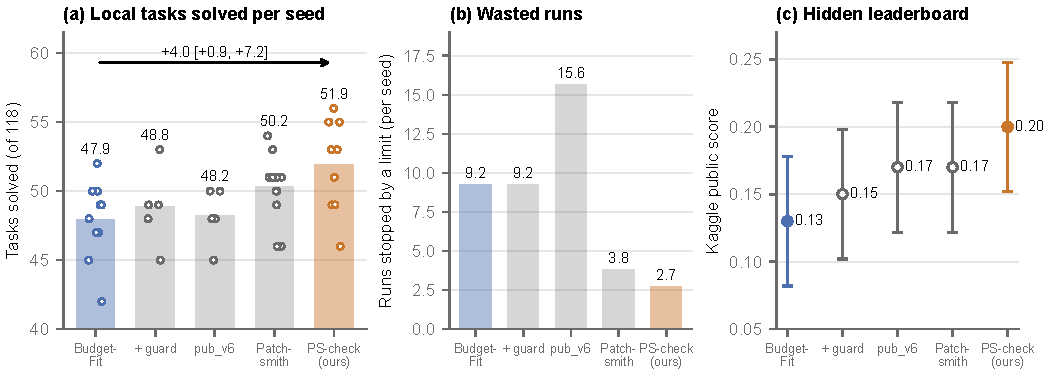
\includegraphics[width=0.92\textwidth]{v2/fig_overview.pdf}
\caption{From the Budget-Fit baseline (blue) to Patchsmith-check (orange). (a) Tasks solved per seed; bars are means, circles single seeds; arrow: paired difference with 95\% CI. (b) Runs per seed stopped by a time, call or turn limit. (c) Hidden public leaderboard; error bars are the SD of the public score across identical submissions by other teams (0.048).}
\label{fig:overview}
\end{figure*}

\subsection{RQ1: one evaluation is noisy}\label{sec:rq1}
Figure~\ref{fig:flip} shows how often each task is solved across 10 seeds of the short regime: about half of the tasks are never solved, a quarter always, and 31 tasks (26\%) flip between seeds. The noise model predicts a per-run SD of 2.35 tasks against 2.85 observed. Table~\ref{tab:noise} gives the consequences: one run's 95\% interval is about $\pm$5 tasks, and even with 5 seeds per arm, differences below 4--5 tasks are not reliably detectable. The leaderboard is noisier still: identical configurations submitted by different teams scored between 0.08 and 0.20 (SD 0.048, $\approx$2.8 of 58 public tasks).

\begin{figure}[t]
\centering
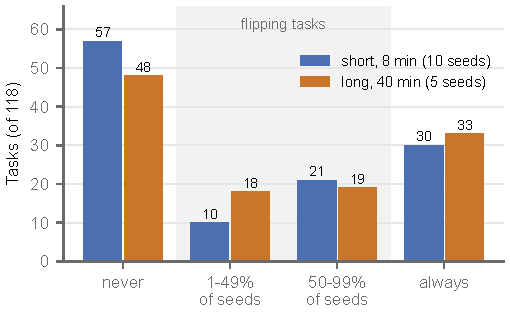
\includegraphics[width=\linewidth]{v2/fig_flip.pdf}
\caption{Tasks grouped by the share of seeds that solve them (short regime, 10 seeds; long regime, 5 seeds). Only the ``flipping'' tasks can be gained by selection, and they make one score noisy.}
\label{fig:flip}
\end{figure}

\begin{table}[t]
\centering
\caption{Seed noise per regime. MDE at 95\% confidence and 80\% power.}
\label{tab:noise}
\begin{tabular}{lcccc}
\toprule
Regime & Mean & SD & 95\% of one run & MDE 3 / 5 seeds\\
\midrule
short & 47.9 & 2.9 & $\pm$4.6 & 5.4 / 4.2\\
medium & 52.8 & 4.1 & $\pm$5.7 & 6.6 / 5.1\\
long & 52.8 & 3.4 & $\pm$5.8 & 6.8 / 5.3\\
long + prompt & 54.8 & 1.1 & $\pm$5.3 & 6.2 / 4.8\\
\bottomrule
\end{tabular}
\end{table}

\subsection{RQ2: spend compute on budget, not samples}\label{sec:rq2}
Figure~\ref{fig:frontier} plots tasks solved against measured cost. The short-run curve lies below the other regimes at every cost. One medium run (5.7\,min) and one long run (7.3\,min) both solve 52.8 tasks; two short runs plus the selector cost 7.6\,min and solve 51.5; five short runs plus the selector cost 19.0\,min (2.6$\times$ a long run) and solve 53.9, not clearly more than one long run ($-1.1$ [$-4.7$, $+2.6$]). Medium$\times$1 beats short$\times$1 by $+4.9$ [$+1.6$, $+8.5$].

\begin{figure}[t]
\centering
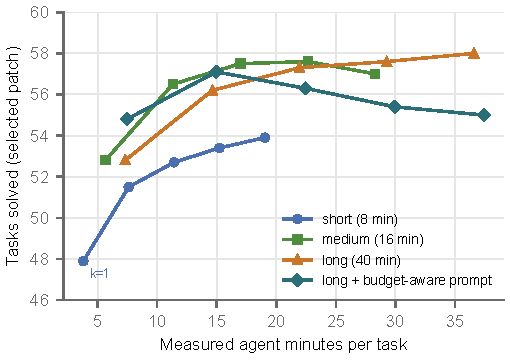
\includegraphics[width=\linewidth]{v2/fig_frontier.pdf}
\caption{Matched-cost frontier: tasks solved vs.\ measured minutes per task for $k=1\ldots5$ runs per task with the frozen selector.}
\label{fig:frontier}
\end{figure}

\emph{Mechanism.} A run is \emph{invalid} if its patch changes no source file or it hits a limit; invalid runs never resolved a task. Their share falls from 20\% (short) to 9\% (medium) and 4\% (long). The extra budget is mostly unused --- the median long run stops after 4.5\,min and 29 calls, and only 14 of 590 long runs hit a limit --- so a 5$\times$ larger budget costs only 1.9$\times$ more. A larger budget acts as insurance for the few tasks that need it.

\emph{Selection does not generalise.} The best in-sample rule (validity filter, then a successful last command after the final edit, then the smallest patch) recovered 72\% of the oracle headroom at $k=5$ ($+7.6$ tasks). On the pre-registered holdout seeds it recovered 34--46\% and was indistinguishable from the validity filter alone (51.0 vs.\ 50.8; Fig.~\ref{fig:holdout}). Gemma~4 judging its own patches added nothing (listwise 62\% of headroom, equal to patch size alone). At $k=5$, long runs contain a correct patch for 70 tasks, but the best selector finds 58: \emph{selection, not generation, is the bottleneck.} Raising one limit alone on an 8-minute agent did not help either (9\,min: $-0.7$; 36 calls: $+0.7$, both n.s.), because failures moved from the call limit to the time limit.

\begin{figure}[t]
\centering
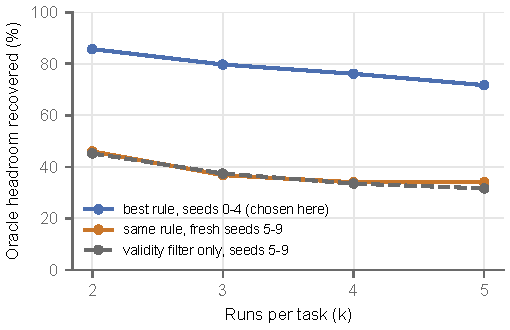
\includegraphics[width=\linewidth]{v2/fig_holdout.pdf}
\caption{Share of oracle headroom recovered by test-free selectors in-sample (seeds 0--4) and on pre-registered holdout seeds (5--9).}
\label{fig:holdout}
\end{figure}

\subsection{RQ3: LoRA on successful trajectories hurts}\label{sec:rq3}
Table~\ref{tab:lora} and Fig.~\ref{fig:lora} summarise the three adapters, each against its matched base on the same serving build.

\begin{table}[t]
\centering
\caption{LoRA adapters vs.\ matched base (3 seeds). $\Delta$ with 95\% paired-bootstrap CI; held-out = 24 tasks excluded from training.}
\label{tab:lora}
\setlength{\tabcolsep}{3pt}
\begin{tabular}{lccc}
\toprule
Configuration & Solved & $\Delta$ [95\% CI] & Held-out\\
\midrule
31B base & 49.0 & & 14.0\\
31B + self LoRA & 46.3 & $-2.7$ [$-7.3$, $+2.0$] & 11.3 ($-2.7^{*}$)\\
31B + Qwen LoRA & 26.3 & $-22.7$ [$-29.7$, $-16.0$] & 6.7\\
\midrule
E4B base (12\,min/40 calls) & 19.0 & & 7.0\\
E4B + 31B LoRA & 10.3 & $-8.7$ [$-14.3$, $-3.0$] & 1.7\\
\bottomrule
\multicolumn{4}{l}{\footnotesize $^{*}$Held-out CI [$-5.7$, $-0.3$] excludes zero.}
\end{tabular}
\end{table}

\begin{figure*}[t]
\centering
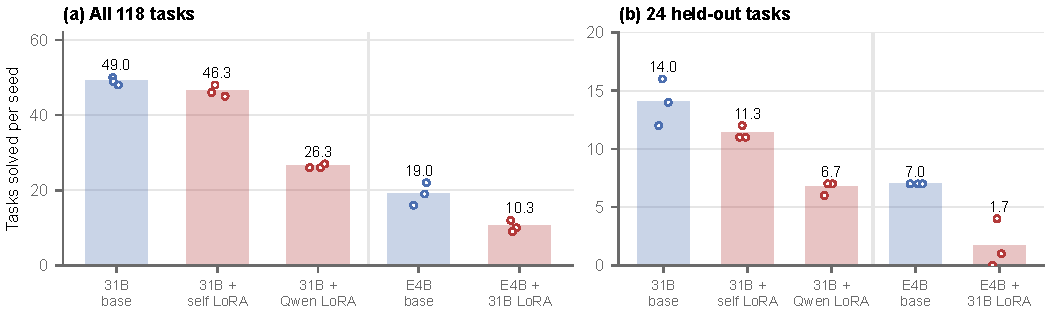
\includegraphics[width=0.8\textwidth]{v2/fig_lora.pdf}
\caption{LoRA adapters (red) vs.\ their matched base (blue), 3 seeds each. (a) All 118 tasks; (b) the 24 tasks held out from training. Bars are means, circles single seeds.}
\label{fig:lora}
\end{figure*}

\emph{Self-training teaches nothing new.} The self adapter matched the base on the 46 tasks it trained on (34.7 vs.\ 35.0) --- the base already solved them 76\% of the time --- and lost 2.7 held-out tasks. Its behaviour changed (first edit at call 9 vs.\ 13; fewer runs without a patch, 10.3 vs.\ 20.7 per seed), but more patches were not more correct patches.

\emph{The teacher's style broke the tool protocol.} The Qwen-distilled adapter called \texttt{submit\_patch} 4.4 times per task (base 1.1); 1,410 of its 1,550 submissions found an unedited tree, burning the call budget, although no training episode ever submits before editing. Its loss fell from 1.02 to 0.38 while it learned this, illustrating that a falling loss does not certify agent behaviour~\cite{gudibande2023false}.

\emph{Down-distillation produced thinking loops.} The E4B adapter's median step length was normal (223 vs.\ 205 tokens) but its mean was 1,528 vs.\ 478: 2,527 steps ended at exactly the 4,096-token thinking budget, against 6 for the base (Fig.~\ref{fig:steps}), with sentences repeated until the cut~\cite{holtzman2020degeneration}. 88 of 118 runs per seed timed out. A label audit (stop tokens, windowing, template) found no bug. LoRA also cost E4B 23\% of generation throughput and 52\% more time per task.

\begin{figure}[t]
\centering
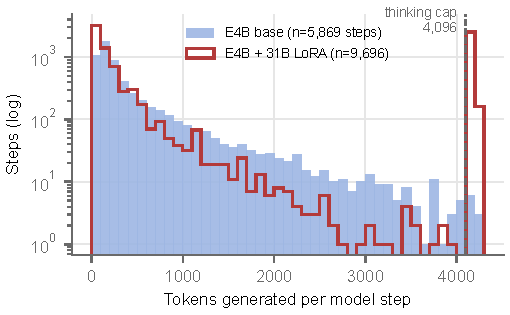
\includegraphics[width=\linewidth]{v2/fig_steps.pdf}
\caption{Tokens generated per model step, E4B base vs.\ E4B with the 31B-trained adapter. The spike at 4,096 is the thinking budget cutting off repetition loops.}
\label{fig:steps}
\end{figure}

\subsection{RQ4: a trace-guided prompt change transfers}\label{sec:rq4}
\emph{Where Patchsmith fails.} Of unsolved runs with a patch, 29\% edit the wrong file, 11\% the right file but the wrong function, and 61\% the right function --- most failures are wrong \emph{implementations}, not wrong locations. The manual audit (Fig.~\ref{fig:audit}) attributes 8 of 30 failures to under-specified issues whose hidden tests expect an API not named in the issue, 6 to flawed implementations, and 7 to process faults that a final check could catch (missed verification, edit-tool loops).

\begin{figure}[t]
\centering
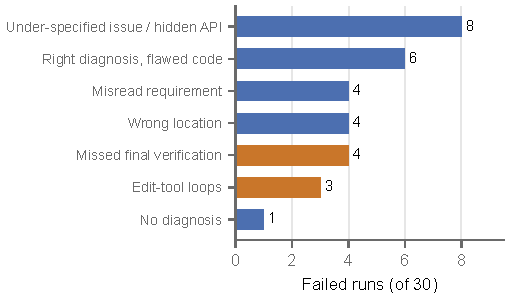
\includegraphics[width=\linewidth]{v2/fig_audit.pdf}
\caption{Manual audit of 30 failed Patchsmith runs (stratified by repository and seed). Orange: process failures targeted by Patchsmith-check.}
\label{fig:audit}
\end{figure}

\emph{What separates solved from failed runs of the same task.} On the 29 mixed tasks, the strongest separator is a behaviour check (test or reproduction) after the \emph{last} edit: present in 88\% of solved vs.\ 47\% of failed runs, $d_z=+0.89$, positive in 20 of 24 tasks. Solved runs also edit earlier (call 13.1 vs.\ 16.7). Reproducing the bug \emph{before} editing does not separate outcomes within task (0.53 vs.\ 0.50), although it correlates with success \emph{between} tasks (64\% vs.\ 38\%) --- a reminder that naive correlations are confounded by task difficulty. Pytest worked in the sandbox (94 of 134 calls exited 0) yet was the final check in only 8\% of runs, because the public prompt warned that ``the sandbox may disable pytest''. Scratch files appeared in 18\% of patches but had no within-task effect ($+0.03$ [$-0.15$, $+0.22$]).

\emph{Result.} Table~\ref{tab:pscheck} and Fig.~\ref{fig:pscheck}. The 3-seed screen passed all gates ($+3.8$ [$+0.3$, $+7.3$], 221\,s/task). On the six fresh confirmation seeds the gain shrank to $+0.8$ [$-2.2$, $+4.0$] --- the expected regression after selecting on a screen --- and the pre-registered pooled comparison was $+1.6$ [$-0.8$, $+4.2$], narrowly above the $+1.5$ bar, with held-out tasks $+0.5$ and a projected Kaggle time of 8.7\,h. The targeted behaviours changed as intended on fresh seeds: pytest as the final check rose from 9\% to 27\% of runs (failed runs: 5\%$\rightarrow$19\%), post-edit checking from 70\% to 74\%, and patches with scratch files fell from 17\% to 1\%. The edit-retry rule had no effect (edit loops 100 vs.\ 111 runs). With pytest disabled, the change cost $-0.8$ tasks and never retried pytest. On Kaggle's hidden tasks the submission completed cleanly and scored \textbf{0.20}, against 0.17 for Patchsmith --- the best of our five submissions (Fig.~\ref{fig:overview}c).

\begin{table}[t]
\centering
\caption{Patchsmith-check vs.\ Patchsmith (118 tasks).}
\label{tab:pscheck}
\setlength{\tabcolsep}{3.5pt}
\begin{tabular}{lccc}
\toprule
Comparison & PS & PS-check & $\Delta$ [95\% CI]\\
\midrule
Screen (6 vs.\ 3 seeds) & 50.8 & 54.7 & $+3.8$ [$+0.3$, $+7.3$]\\
Fresh seeds 6--11 & 49.7 & 50.5 & $+0.8$ [$-2.2$, $+4.0$]\\
Pooled (12 vs.\ 9 seeds) & 50.2 & 51.9 & $+1.6$ [$-0.8$, $+4.2$]\\
Pooled held-out & 14.5 & 15.0 & $+0.5$ [$-1.4$, $+2.5$]\\
Seconds per task & 218 & 222 & \\
Kaggle public score & 0.17 & \textbf{0.20} & \\
\bottomrule
\end{tabular}
\end{table}

\begin{figure*}[t]
\centering
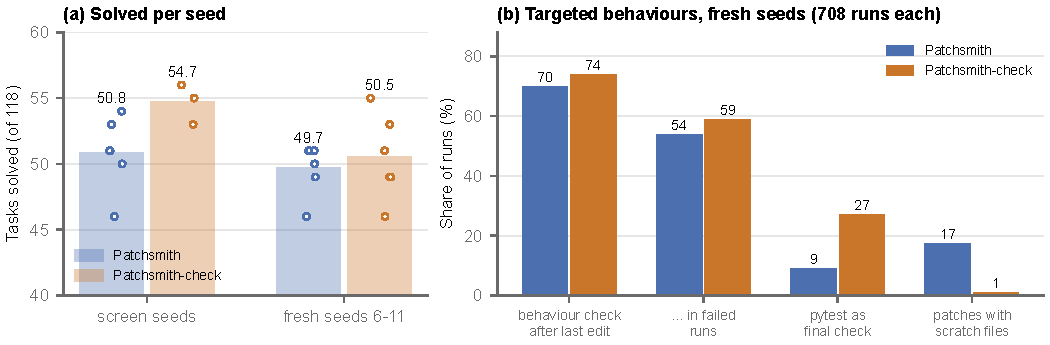
\includegraphics[width=0.85\linewidth]{v2/fig_pscheck.pdf}
\caption{Patchsmith-check. (a) Tasks solved per seed on screen and fresh seeds. (b) Behaviour on the fresh seeds: the targeted checks rise, scratch files disappear.}
\label{fig:pscheck}
\end{figure*}


\emph{Other agent designs did not help.} Table~\ref{tab:neg} lists design changes evaluated with the same protocol. None improved the agent: adding budget, parallel solvers, helper scripts, a reviewer stage, a larger or smaller thinking budget, or sampling changes all lost or tied, mostly by moving failures from one limit to another or by slowing the agent. A final round on top of Patchsmith-check confirms this: a reviewer agent raised timeouts from 23 to 36 per seed and left scratch files in 43 of 354 patches, and a larger thinking budget raised timeouts from 23 to 33.

\begin{table}[t]
\centering
\caption{Other levers (3 seeds each unless noted; $\Delta$ vs.\ matched baseline).}
\label{tab:neg}
\setlength{\tabcolsep}{3pt}
\begin{tabular}{llc}
\toprule
Change & Model & $\Delta$ [95\% CI]\\
\midrule
Temperature 1.0 & 31B & $+0.3$ [$-4.3$, $+5.0$]\\
Frequency penalty 0.2 & 31B & $-3.0$ [$-7.7$, $+1.7$]\\
Thinking budget 2,048 & 31B & $-1.0$ [$-5.0$, $+3.0$]\\
Code-search/test-finder skill scripts & 31B & $-1.7$ [$-5.3$, $+2.0$]\\
3 parallel solvers + selector (16\,min) & 31B & $\pm0$, 4$\times$ slower\\
Patchsmith, 9\,min / 32 calls & 31B & $-1.5$ [$-5.0$, $+2.2$]\\
Minimal 3-tool agent, thinking 256 & 31B & $-2.7$\\
Solver + reviewer (SequentialAgent) & E4B & $-1.3$ [$-5.7$, $+3.0$]\\
Thinking off & E4B & $-5.3$ [$-8.7$, $-2.0$]\\
\midrule
\multicolumn{3}{l}{\emph{On top of Patchsmith-check (1 GPU, matched baseline 51.3):}}\\
Spec-coverage checklist step & 31B & $-1.0$ [$-5.3$, $+3.3$]\\
Solver + reviewer (SequentialAgent) & 31B & $-4.0$ [$-8.7$, $+0.7$]\\
Thinking budget 8,192 & 31B & $-3.0$ [$-7.7$, $+1.3$]\\
\bottomrule
\end{tabular}
\end{table}

%=========================================================
\section{Discussion}
\paragraph*{What produced the improvement} The path from 0.13 to 0.20 did not come from more compute, more samples or new weights: all three were tested and failed (RQ2, RQ3, Table~\ref{tab:neg}). It came from two agent-design changes that reduce wasted runs and unverified patches --- a stronger workflow that reaches an edit and a check within the budget, and our evidence-driven correction of it. Both act on the failure mode that the noise and budget analyses identify.

\paragraph*{Why budget beats samples} For a small agent, the dominant failure is not a wrong idea but a \emph{wasted run}: no patch, a budget hit or an edit loop. A larger budget removes these runs at little cost because most runs stop early anyway, whereas sampling multiplies them and leaves a selector that, without tests, cannot reliably tell good patches from bad ones. Test-time scaling results from large models~\cite{brown2024monkeys,ehrlich2025codemonkeys} rely on a verifier that a small local agent does not have.

\paragraph*{Why fine-tuning failed} Our datasets contain 126--169 episodes from at most 46 tasks, two orders of magnitude fewer distinct tasks than SWE-Gym or SWE-smith~\cite{pan2025swegym,yang2025swesmith}. Self-training on tasks the model already solves mostly reinforces what it knows~\cite{zelikman2022star}, and the two distillation settings show the classical failure modes of imitation --- copying a teacher's surface protocol~\cite{gudibande2023false} and degenerate repetition in a smaller student~\cite{holtzman2020degeneration}. Under a wall-clock budget, LoRA's serving overhead must also be paid for before any gain shows.

\paragraph*{Why the prompt change worked} Patchsmith-check did not add capability; it removed a false belief (``pytest may be disabled'') that suppressed the most predictive behaviour, a final behavioural check. The within-task design was essential: the intuitive ``reproduce first'' advice is a between-task artefact. The effect is small ($\approx$+1 task on fresh seeds) and within leaderboard noise, which is why we relied on behavioural metrics and pre-registered gates rather than on the public score.

\paragraph*{Local vs.\ hidden tasks} The same agents solve about 44\% of local tasks but 17--20\% of the public leaderboard tasks. A 26-task Kaggle run matched our predicted solve rate on the public tasks, so the gap reflects harder hidden tasks rather than hardware. Local and leaderboard scores agree on the overall trend (our two best local agents are our two best submissions), but individual leaderboard differences between configurations within $\approx$2 local tasks of each other are not interpretable (Fig.~\ref{fig:overview}c).

\paragraph*{Limitations and threats to validity} (1) One model family, four repositories, two of which make up 89\% of tasks. (2) Holdouts are over seeds (RQ2) and over solvable tasks (RQ3), not new repositories. (3) We ran on H100 rather than L4 and project runtime with a measured 1.17$\times$ factor. (4) Three to twelve seeds leave differences of 1--2 tasks unresolved; the Patchsmith-check gain on fresh seeds alone is not statistically significant. (5) The LoRA results bound what a competition-sized dataset can do, not what fine-tuning can do in general.

%=========================================================
\section{Conclusion}
Starting from the public Budget-Fit agent, we improved a Gemma~4 coding agent from 47.9 to 51.9 local tasks ($+4.0$ [$+0.9$, $+7.2$]) and from 0.13 to 0.20 on the hidden leaderboard, within the same compute budget. For a small open-weight coding agent under a hard compute budget, the levers that are popular for frontier models do not transfer directly. Repeated sampling without a verifier and LoRA fine-tuning on a few hundred trajectories both failed in controlled tests, while a larger per-run budget and a small, evidence-driven prompt change helped. The common thread is measurement: one run carries $\pm$5 tasks of noise, in-sample selection rules and screen results shrink on fresh seeds, and behaviour metrics computed from traces explain results that scores alone cannot. We recommend that agent developers (i) count measured rather than nominal cost, (ii) use 3--5 seeds with paired tests and a screen--confirm protocol, (iii) audit tool-protocol statistics and thinking-budget hits before trusting a fine-tuned adapter, and (iv) derive agent changes from within-task contrasts of solved and failed traces. Code and per-run results: \url{https://github.com/HRDevelops/gemma4-compute-allocation}.

\bibliographystyle{IEEEtran}
\bibliography{refs}
\end{document}
